\documentclass[11pt,a4paper]{article}
\usepackage[utf8]{inputenc}
\usepackage[T1]{fontenc}
\usepackage[spanish,es-noshorthands,es-nodecimaldot]{babel}
\usepackage{lmodern}
\usepackage[margin=2.4cm]{geometry}
\usepackage{amsmath,amssymb,amsthm,mathtools}
\usepackage{graphicx}
\usepackage{booktabs}
\usepackage{enumitem}
\usepackage[most]{tcolorbox}
\usepackage{xcolor}
\usepackage[colorlinks=true,linkcolor=blue!50!black,urlcolor=blue!50!black,citecolor=blue!50!black]{hyperref}
\usepackage{microtype}

\definecolor{clave}{HTML}{1F4E9C}
\newtcolorbox{idea}[1][Idea clave]{enhanced,colback=clave!5,colframe=clave!70,
  fonttitle=\bfseries\small,title={#1},boxrule=0.6pt,arc=2pt,left=6pt,right=6pt,top=4pt,bottom=4pt}

\theoremstyle{definition}
\newtheorem{definicion}{Definición}[section]
\newtheorem{ejemplo}{Ejemplo}[section]
\theoremstyle{plain}
\newtheorem{proposicion}{Proposición}
\newtheorem{lema}{Lema}[section]

\newcommand{\etaC}{\eta_{\mathrm{C}}}
\newcommand{\Pmax}{P_{\max}}
\newcommand{\dd}{\mathrm{d}}
\newcommand{\code}[1]{\texttt{\small #1}}

\setlength{\parskip}{0.35em}
\setlist{itemsep=0.15em,topsep=0.3em}

\title{\textbf{Guía de estudio}\\[0.3em]
\large Motores de Otto cuánticos, fluctuaciones y la geometría del frente de Pareto\\[0.2em]
\normalsize Qué hicimos, por qué funciona y cómo se conecta con termodinámica y mecánica estadística}
\author{Hugo Campos}
\date{Noviembre de 2026}

\begin{document}
\maketitle

\begin{abstract}
\noindent Esta guía explica, desde cero y con todas las derivaciones, el proyecto
\code{hidden-front} (antes \code{otto-cuantico-awa}) y el borrador de paper que salió de él. Empieza por la física de un qubit
en contacto con un baño, construye el ciclo de Otto en tiempo finito, calcula la estadística
completa del trabajo con una matriz inclinada, introduce la producción de entropía y la relación de
incertidumbre termodinámica (TUR), y llega al resultado central: la forma (convexa o de silla) del
frente de Pareto depende de si se usa la eficiencia $\eta$ o la producción de entropía $\Sigma$ como
objetivo, y eso decide qué motores puede encontrar una figura de mérito lineal. Al final hay un
mapa del código, una sección honesta sobre qué es nuevo y qué no, y ejercicios resueltos.
\end{abstract}

\tableofcontents
\clearpage

%======================================================================
\section{El panorama en una página}
%======================================================================

\paragraph{La pregunta.} Un motor térmico microscópico tiene tres cosas que nos importan:
\begin{itemize}
\item su \textbf{potencia} media $P$ (cuánto trabajo entrega por unidad de tiempo),
\item su \textbf{eficiencia} $\eta$ (qué fracción del calor absorbido convierte en trabajo), o
  equivalentemente su \textbf{producción de entropía} $\Sigma$ (cuánto disipa),
\item sus \textbf{fluctuaciones de potencia} $\Delta P$ (qué tan irregular es la entrega).
\end{itemize}
No se pueden optimizar las tres a la vez: hay un compromiso. El conjunto de los mejores
compromisos es el \textbf{frente de Pareto}.

\paragraph{La práctica habitual.} Para encontrar el frente, muchos trabajos maximizan una
\emph{figura de mérito lineal}, por ejemplo $F = aP + b\eta - c\,\Delta P$, y barren los pesos
$(a,b,c)$. Cada elección de pesos da un motor óptimo; juntándolos se espera obtener el frente.

\paragraph{El problema.} Una suma ponderada solo puede encontrar los puntos del frente que están en
su envolvente convexa (los \emph{puntos soportados}). Si el frente tiene partes no convexas, la suma
ponderada no las ve, \emph{con ningún peso}.

\paragraph{Lo que mostramos.}
\begin{enumerate}
\item Si el frente satura la TUR (la cota de precisión que impone la segunda ley) y es una superficie
  (potencia y eficiencia se ajustan por separado), entonces en las variables $(P,\eta,\Delta P)$ el
  frente es una \textbf{silla de montar}: ningún punto interior es soportado.
\item Los \emph{mismos motores}, descritos con $(P,\Delta P,\Sigma)$, forman una superficie
  \textbf{convexa} (un ``tazón''): todos los puntos son soportados.
\item En un motor de Otto de un qubit, que satura la TUR, la suma ponderada con $\eta$ alcanza solo
  el $11\%$ del frente y pierde en mediana un $14\%$ en algún objetivo; con $\Sigma$ no pierde nada en
  la mediana.
\item En respuesta lineal (cerca del equilibrio) el frente es una curva y la suma ponderada funciona;
  con control muy libre la TUR se rompe y la silla desaparece. El efecto está ligado a la saturación.
\end{enumerate}

\begin{idea}
Elegir $\eta$ o $\Sigma$ como objetivo parece una cuestión de gusto, porque a potencia fija
maximizar una es minimizar la otra. Pero la relación entre ellas es no lineal, y una
transformación no lineal de coordenadas puede convertir una superficie convexa en una silla. La
suma ponderada es sensible a esa diferencia; la dominancia de Pareto no.
\end{idea}

\paragraph{Cómo leer esta guía.} Las secciones 2--5 son física (lo que verías en un curso de
termodinámica y mecánica estadística, aplicado a un qubit). Las secciones 6--9 son el resultado. Las
secciones 10--13 son los números, los algoritmos y el código. La sección 14 tiene ejercicios con
soluciones. Unidades: $\hbar = k_B = 1$ en todo el texto.

%======================================================================
\section{Un qubit en contacto con un baño térmico}
%======================================================================

\subsection{El sistema de dos niveles}

Un qubit es el sistema cuántico más simple: dos estados, que llamamos fundamental ($s=0$, energía
$0$) y excitado ($s=1$, energía $\omega$). La diferencia de energía $\omega$ es la \textbf{brecha}
(\emph{gap}). En un qubit superconductor (un transmón, por ejemplo) la brecha se controla desde
afuera con un flujo magnético; por eso tiene sentido pensar en $\omega$ como un parámetro que el
experimentador mueve, igual que el pistón de un motor mueve el volumen.

Como solo hay dos estados, el estado estadístico del qubit (sin coherencias) queda descrito por un
solo número: la \textbf{población excitada} $p$, la probabilidad de encontrarlo en $s=1$.

\subsection{Equilibrio: la distribución de Gibbs}

En equilibrio con un baño a temperatura $T$, el ensamble canónico da
\begin{equation}
p_{\mathrm{eq}} = \frac{e^{-\omega/T}}{1 + e^{-\omega/T}} = \frac{1}{1+e^{\omega/T}} \equiv a(\omega,T).
\label{eq:gibbs}
\end{equation}
Es la misma forma que la distribución de Fermi--Dirac (con potencial químico nulo), porque un nivel
que está ocupado o vacío es matemáticamente lo mismo que un qubit excitado o no. La población
excitada depende solo del cociente $\omega/T$: brecha grande o baño frío $\Rightarrow$ $a \to 0$;
brecha chica o baño caliente $\Rightarrow$ $a \to 1/2$ (Fig.~\ref{fig:poblacion}).

\begin{figure}[h]
\centering
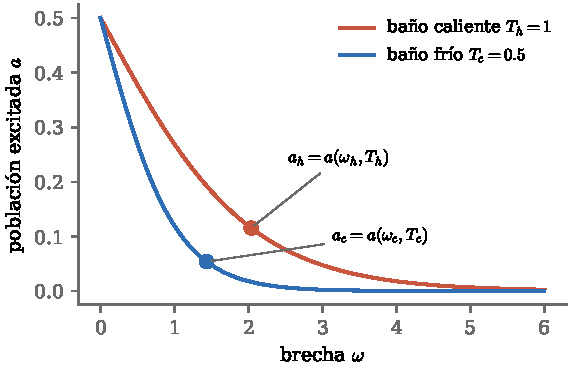
\includegraphics[width=0.62\linewidth]{figs/poblacion.pdf}
\caption{Población excitada de equilibrio $a(\omega,T)$ para los dos baños del proyecto
($T_h = 1$, $T_c = 0.5$). Los puntos marcan las brechas del motor de potencia máxima
($\omega_h = 2.04$, $\omega_c = 1.43$): aunque $\omega_h > \omega_c$, el baño caliente deja más
población excitada, $a_h > a_c$. Esa desigualdad es lo que hace funcionar el motor.}
\label{fig:poblacion}
\end{figure}

\subsection{Fuera del equilibrio: la ecuación maestra}

Si el qubit no está en equilibrio, el baño lo empuja hacia él. El modelo más simple es una
\textbf{ecuación maestra} con tasas de excitación $k_+$ y de decaimiento $k_-$:
\begin{equation}
\dot p = k_+(1-p) - k_-\,p .
\end{equation}
Para que el estado estacionario sea el de Gibbs, las tasas deben cumplir \textbf{balance detallado},
$k_+/k_- = e^{-\omega/T}$. Definiendo la tasa total $\gamma = k_+ + k_-$, la ecuación queda
\begin{equation}
\dot p = -\gamma\,\bigl(p - a(\omega,T)\bigr)
\qquad\Longrightarrow\qquad
p(t) = a + \bigl(p(0) - a\bigr)e^{-\gamma t}.
\label{eq:relax}
\end{equation}
La población relaja exponencialmente hacia $a$ con tiempo característico $1/\gamma$. En el proyecto
$\gamma = 1$, así que los tiempos están medidos en unidades de $1/\gamma$.

\subsection{La matriz de transición de un contacto}

Para la estadística necesitamos más que $p$: necesitamos la probabilidad de \emph{saltar} de un
estado a otro durante un contacto de duración $\tau$. Con $x = e^{-\gamma\tau}$ y la
ec.~\eqref{eq:relax}:
\begin{itemize}
\item si empieza en $s=0$ ($p(0)=0$), termina excitado con probabilidad $a(1-x)$;
\item si empieza en $s=1$ ($p(0)=1$), termina excitado con probabilidad $a + (1-a)x$, es decir,
  termina abajo con probabilidad $(1-a)(1-x)$.
\end{itemize}
Eso define la matriz estocástica (filas: estado inicial; columnas: estado final)
\begin{equation}
M = \begin{pmatrix} 1 - a(1-x) & a(1-x) \\ (1-a)(1-x) & 1 - (1-a)(1-x)\end{pmatrix},
\qquad \det M = x .
\label{eq:M}
\end{equation}
Esto es \code{relaxation\_matrix} en \code{otto/model.py}. Que $\det M = x$ (no depende de $a$)
será importante más adelante.

%======================================================================
\section{El ciclo de Otto cuántico}
%======================================================================

\subsection{Los cuatro tramos}

El ciclo de Otto de un motor a gasolina tiene dos adiabáticas (compresión y expansión) y dos
isocoras (calentamiento y enfriamiento a volumen fijo). En el Otto cuántico, la brecha $\omega$ hace
el papel del volumen:
\begin{enumerate}
\item \textbf{Isocora caliente.} Brecha fija $\omega_h$, contacto con el baño caliente $T_h$ durante
  $\tau_h$. La población sube de $p_2$ a $p_1$.
\item \textbf{Adiabática (quench).} Se desconecta el baño y se cambia la brecha $\omega_h\to\omega_c$
  en un tiempo $\tau_q$, tan rápido que la población no cambia.
\item \textbf{Isocora fría.} Brecha $\omega_c$, contacto con el baño frío $T_c$ durante $\tau_c$. La
  población baja de $p_1$ a $p_2$.
\item \textbf{Adiabática de vuelta}, $\omega_c\to\omega_h$, otra vez a población fija.
\end{enumerate}

\subsection{Calor y trabajo: la primera ley microscópica}

La energía media del qubit es $E = \sum_s \varepsilon_s p_s = \omega\,p$. Su diferencial tiene dos
términos:
\begin{equation}
\dd E = \underbrace{\sum_s \varepsilon_s\,\dd p_s}_{\text{calor}} \;+\;
\underbrace{\sum_s p_s\,\dd\varepsilon_s}_{\text{trabajo}}
\;=\; \omega\,\dd p + p\,\dd\omega .
\end{equation}
Cambiar las \emph{probabilidades} con los niveles fijos es intercambiar calor con el baño; cambiar
los \emph{niveles} con las probabilidades fijas es hacer trabajo. Es exactamente la separación que
usa la termodinámica cuántica, y en el Otto los tramos la separan limpiamente
(Fig.~\ref{fig:ciclo}, izquierda):
\begin{align}
Q_h &= \omega_h\,(p_1 - p_2) &&\text{(calor absorbido del baño caliente)}\\
Q_c &= \omega_c\,(p_1 - p_2) &&\text{(calor entregado al baño frío)}\\
W   &= Q_h - Q_c = (\omega_h - \omega_c)(p_1 - p_2) &&\text{(trabajo extraído por ciclo)}
\end{align}

\begin{figure}[h]
\centering
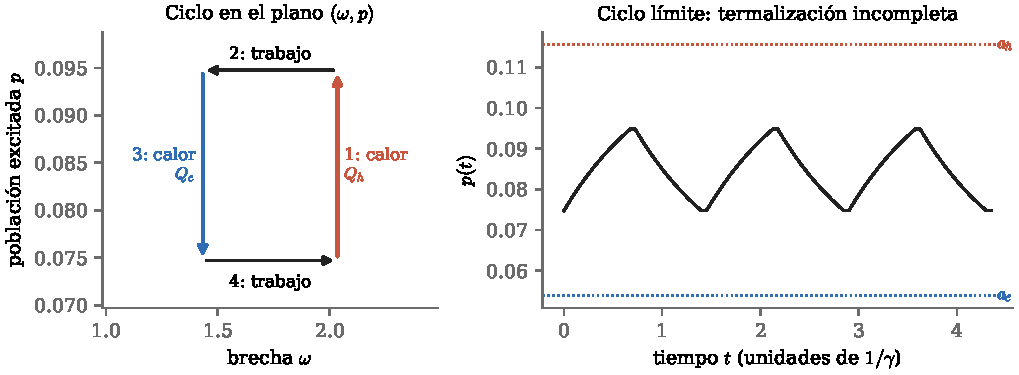
\includegraphics[width=\linewidth]{figs/ciclo.pdf}
\caption{Izquierda: el ciclo de Otto en el plano $(\omega,p)$ para el motor de potencia máxima; el
área encerrada es el trabajo $W$. Derecha: la población $p(t)$ durante tres ciclos. Nunca llega a
$a_h$ ni a $a_c$: la termalización es incompleta. Después de unos pocos ciclos el qubit entra en un
\emph{ciclo límite} y $p$ oscila entre $p_2$ y $p_1$.}
\label{fig:ciclo}
\end{figure}

\subsection{Eficiencia de Otto y la condición para ser motor}

Dividiendo,
\begin{equation}
\eta = \frac{W}{Q_h} = 1 - \frac{\omega_c}{\omega_h}.
\label{eq:etaotto}
\end{equation}
La eficiencia depende \emph{solo} del cociente de brechas $r = \omega_c/\omega_h$, no de los tiempos.
Para que el ciclo sea un motor ($W > 0$) necesitamos $p_1 > p_2$, lo que (como veremos) requiere
$a_h > a_c$:
\begin{equation}
\frac{1}{1+e^{\omega_h/T_h}} > \frac{1}{1+e^{\omega_c/T_c}}
\iff \frac{\omega_h}{T_h} < \frac{\omega_c}{T_c}
\iff r > \frac{T_c}{T_h}
\iff \eta < 1 - \frac{T_c}{T_h} = \etaC .
\end{equation}
La segunda ley aparece sola: el Otto nunca supera a Carnot. Por eso en el código la variable
$r$ vive en $[T_c/T_h,\,1]$: con $r = T_c/T_h$ se tiene $\eta = \etaC$ (pero potencia nula), y con
$r = 1$ se tiene $\eta = 0$.

\subsection{Tiempo finito: el ciclo límite}

Con contactos de duración finita, $x_h = e^{-\gamma\tau_h}$ y $x_c = e^{-\gamma\tau_c}$ son distintos
de cero y el qubit no termaliza. Aplicando \eqref{eq:relax} a cada contacto,
\begin{equation}
p_1 = a_h + (p_2 - a_h)x_h, \qquad p_2 = a_c + (p_1 - a_c)x_c .
\end{equation}
Resolviendo el sistema (ejercicio~\ref{ej:ciclolimite}):
\begin{equation}
\boxed{\;p_1 - p_2 = \frac{(a_h - a_c)(1-x_h)(1-x_c)}{1 - x_h x_c}\;}
\label{eq:dp}
\end{equation}
Esta fórmula lo explica casi todo:
\begin{itemize}
\item el signo lo pone $a_h - a_c$: hay motor si y solo si $r > T_c/T_h$;
\item los factores $(1-x)$ castigan los contactos cortos: si $\tau\to 0$, $x\to1$ y no hay
  intercambio de calor;
\item la potencia es $P = W/\tau_{\mathrm{ciclo}}$ con $\tau_{\mathrm{ciclo}} = \tau_h + \tau_c + 2\tau_q$,
  que castiga los contactos largos.
\end{itemize}
Entre ambos extremos hay un óptimo: el \textbf{compromiso potencia--eficiencia}.

\begin{ejemplo}[El motor de potencia máxima]
Con $T_h = 1$, $T_c = 0.5$, $\gamma = 1$ y $\tau_q = 0.05$, el máximo de potencia está en
$\omega_h \approx 2.035$, $r \approx 0.704$ ($\omega_c \approx 1.433$), $\tau_h \approx \tau_c \approx 0.675$.
Ahí:
\begin{center}
\begin{tabular}{lll}
\toprule
$a_h = 0.116$, $a_c = 0.054$ & $p_1 = 0.0948$, $p_2 = 0.0747$ & $\tau_{\mathrm{ciclo}} = 1.450$ \\
$W = 0.0121$ por ciclo & $P = 0.00833$ & $\eta = 0.296$ \\
$\Delta P = 0.0126$ & $\Sigma = 0.0115$ & $\xi = 0.96$ \\
\bottomrule
\end{tabular}
\end{center}
La eficiencia a potencia máxima, $0.296$, es casi la de \textbf{Curzon--Ahlborn},
$1-\sqrt{T_c/T_h} = 0.293$. Fue la primera verificación de que el modelo se comporta como un motor
físico razonable. ($\Delta P$, $\Sigma$ y $\xi$ se definen en las secciones siguientes.)
\end{ejemplo}

%======================================================================
\section{Termodinámica estocástica: el trabajo fluctúa}
%======================================================================

\subsection{Un solo qubit no tiene ``población 0.09''}

Hasta aquí usamos promedios. Pero un qubit individual está, en cada instante, arriba o abajo. Al
hacer el primer quench, si está excitado ($s_1 = 1$) entrega $\Delta\omega = \omega_h - \omega_c$ de
trabajo; si está abajo, nada. En el segundo quench, si está excitado ($s_2 = 1$) hay que pagar
$\Delta\omega$. El trabajo de un ciclo es una \textbf{variable aleatoria}:
\begin{equation}
w = \Delta\omega\,(s_1 - s_2) \in \{-\Delta\omega,\ 0,\ +\Delta\omega\}.
\end{equation}
Su media es $\langle w\rangle = \Delta\omega(p_1 - p_2) = W$, pero en un ciclo dado puede ser
negativa. Esta es la idea central de la \emph{termodinámica estocástica}: calor, trabajo y entropía
se definen trayectoria por trayectoria y fluctúan; las leyes de la termodinámica valen para los
promedios (y, más finamente, para las distribuciones).

\subsection{Qué queremos medir}

Tras $n$ ciclos el trabajo acumulado es $W_n = \sum_{k=1}^n w_k$. Para $n$ grande,
\begin{equation}
\langle W_n\rangle \simeq n\,\langle w\rangle, \qquad
\operatorname{Var}(W_n) \simeq n\,v ,
\end{equation}
y definimos la \textbf{potencia} y las \textbf{fluctuaciones de potencia} como tasas:
\begin{equation}
P = \frac{\langle w\rangle}{\tau_{\mathrm{ciclo}}}, \qquad
\Delta P = \lim_{t\to\infty}\frac{\operatorname{Var}(W_t)}{t} = \frac{v}{\tau_{\mathrm{ciclo}}} .
\end{equation}
$\Delta P$ es un coeficiente de difusión: mide cuánto se abre el abanico de trayectorias
(Fig.~\ref{fig:tray}).

\begin{figure}[h]
\centering
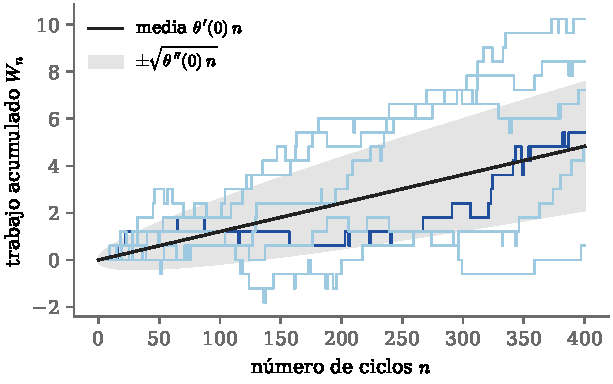
\includegraphics[width=0.66\linewidth]{figs/trayectorias.pdf}
\caption{Seis trayectorias simuladas del trabajo acumulado en el motor de potencia máxima. Todas
crecen en promedio con pendiente $\theta'(0)$, pero se separan como $\sqrt{n}$; la banda gris es
$\pm\sqrt{\theta''(0)\,n}$. $P$ es la pendiente por unidad de tiempo; $\Delta P$ es el ancho del
abanico por unidad de tiempo.}
\label{fig:tray}
\end{figure}

\paragraph{La trampa: correlaciones.} Uno estaría tentado de calcular $v = \operatorname{Var}(w)$ de
un ciclo. Pero los ciclos están correlacionados: si un ciclo termina con el qubit excitado, el
siguiente empieza excitado. Entonces $\operatorname{Var}(W_n) \neq n\operatorname{Var}(w)$; hay que
sumar todas las covarianzas entre ciclos. La herramienta que hace esto de una vez es la estadística
de conteo completa.

\subsection{Estadística de conteo completa y la matriz inclinada}

La \textbf{función generadora de momentos} del trabajo acumulado es
$\langle e^{\chi W_n}\rangle$. Como el qubit es una cadena de Markov, esa suma sobre trayectorias
se puede escribir como un producto de matrices. En cada ciclo:
\begin{itemize}
\item se pasa del estado $s$ (al inicio) a $s_1$ con $M^h$, y se acumula el factor
  $e^{\chi\Delta\omega s_1}$ del primer quench;
\item se pasa de $s_1$ a $s'$ con $M^c$, y se acumula $e^{-\chi\Delta\omega s'}$ del segundo quench.
\end{itemize}
Eso define la \textbf{matriz inclinada} (\emph{tilted matrix}) de un ciclo:
\begin{equation}
\mathcal{T}(\chi)_{s s'} = \sum_{s_1\in\{0,1\}} M^h_{s s_1}\,e^{\chi\Delta\omega s_1}\,M^c_{s_1 s'}\,e^{-\chi\Delta\omega s'} ,
\qquad
\langle e^{\chi W_n}\rangle = \pi^{\top}\,\mathcal{T}(\chi)^n\,\mathbf{1} .
\end{equation}
Para $\chi = 0$ es la matriz de transición de un ciclo completo (estocástica, autovalor máximo
$1$). Para $n$ grande, $\mathcal{T}^n$ está dominada por su mayor autovalor $\lambda(\chi)$:
\begin{equation}
\langle e^{\chi W_n}\rangle \asymp \lambda(\chi)^n
\quad\Longrightarrow\quad
\theta(\chi) \equiv \lim_{n\to\infty}\frac{1}{n}\ln\langle e^{\chi W_n}\rangle = \ln\lambda(\chi).
\end{equation}
$\theta$ es la \textbf{función generadora de cumulantes escalada}. Sus derivadas en $\chi=0$ dan los
cumulantes por ciclo, \emph{con todas las correlaciones incluidas}:
\begin{equation}
\langle w\rangle = \theta'(0), \qquad v = \theta''(0).
\end{equation}

\begin{idea}[Analogía con el ensamble canónico]
$\theta(\chi)$ cumple para el trabajo el papel que $\ln Z(\beta)$ cumple para la energía: derivarla
da la media y la varianza. Y, como en mecánica estadística, la probabilidad de observar un trabajo
por ciclo atípico $w$ decae como $e^{-n I(w)}$, donde la ``función de tasa'' $I$ es la
\emph{transformada de Legendre} de $\theta$ (teoría de grandes desviaciones). Volveremos a encontrar
una transformada de Legendre en el resultado central (sección~\ref{sec:legendre}).
\end{idea}

\subsection{Forma cerrada (por qué el cálculo es exacto)}

Una matriz $2\times2$ tiene autovalores que dependen solo de su traza $t(\chi)$ y su determinante
$D(\chi)$:
\begin{equation}
\lambda(\chi) = \tfrac12\Bigl(t + \sqrt{t^2 - 4D}\Bigr).
\end{equation}
\textbf{El determinante no depende de $\chi$.} Como $\det(AB) = \det A\det B$ y los factores
$e^{\pm\chi\Delta\omega s}$ son matrices diagonales que se cancelan en el determinante,
$D = \det M^h\det M^c = x_h x_c$ (por la ec.~\eqref{eq:M}). La traza sí depende de $\chi$:
\begin{equation}
t(\chi) = c_0 + c_+e^{\chi\Delta\omega} + c_-e^{-\chi\Delta\omega},\qquad
c_+ = M^h_{01}M^c_{10},\quad c_- = M^h_{10}M^c_{01}.
\end{equation}
($c_+$: subir en el baño caliente y bajar en el frío, un ciclo ``productivo''; $c_-$: lo contrario.)
Derivando implícitamente $\lambda^2 - t\lambda + D = 0$ y usando $\lambda(0) = 1$, $t(0) = 1 + D$:
\begin{equation}
\lambda'(0) = \frac{t'(0)}{1-D},\qquad
\lambda''(0) = \frac{t''(0)}{1-D} - \frac{2D\,t'(0)^2}{(1-D)^3},
\end{equation}
con $t'(0) = \Delta\omega(c_+ - c_-)$ y $t''(0) = \Delta\omega^2(c_+ + c_-)$. Finalmente
$\theta'(0) = \lambda'(0)$ y $\theta''(0) = \lambda''(0) - \lambda'(0)^2$. Esto es literalmente lo
que hace \code{cycle\_statistics}. Se puede comprobar que $\theta'(0) = \Delta\omega(p_1 - p_2)$,
de acuerdo con la ec.~\eqref{eq:dp}.

\paragraph{Validación.} \code{monte\_carlo\_work} simula miles de qubits saltando con números
aleatorios y estima media y varianza por fuerza bruta. Coinciden con $\theta'(0)$ y $\theta''(0)$
dentro del error estadístico, y las derivadas analíticas coinciden con diferencias finitas de
$\theta$. Esa es la base de confianza de todo lo demás.

%======================================================================
\section{Producción de entropía y la relación de incertidumbre termodinámica}
%======================================================================

\subsection{Producción de entropía}

La entropía del qubit vuelve a su valor inicial en cada ciclo, así que toda la entropía producida
termina en los baños. Por unidad de tiempo:
\begin{equation}
\Sigma = \frac{1}{\tau_{\mathrm{ciclo}}}\left(\frac{Q_c}{T_c} - \frac{Q_h}{T_h}\right) \;\ge\; 0 .
\end{equation}
Es la segunda ley. Usando $Q_h = P\tau/\eta$ y $Q_c = Q_h - W$ (ejercicio~\ref{ej:sigma}):
\begin{equation}
\boxed{\;\Sigma = \frac{P\,(\etaC - \eta)}{\eta\,T_c}\;}
\qquad\Longleftrightarrow\qquad
\eta = \frac{\etaC\,P}{P + T_c\,\Sigma}.
\label{eq:sigma}
\end{equation}
Lectura: $\eta = \etaC$ si y solo si $\Sigma = 0$ (proceso reversible). A potencia fija, maximizar
$\eta$ y minimizar $\Sigma$ son lo mismo. Pero la relación entre ambas es \emph{no lineal}, y eso
será decisivo.

En el modelo de Otto, $\Sigma = (p_1 - p_2)\bigl(\omega_c/T_c - \omega_h/T_h\bigr)/\tau_{\mathrm{ciclo}}$,
que es positivo justamente cuando $r > T_c/T_h$.

\subsection{La relación de incertidumbre termodinámica (TUR)}

La TUR (Barato y Seifert 2015; Gingrich \emph{et al.} 2016) dice que \textbf{la precisión cuesta
disipación}. Para cualquier corriente $J_t$ (algo que se acumula en el tiempo, como el trabajo) de un
proceso de Markov estacionario,
\begin{equation}
\frac{\operatorname{Var}(J_t)}{\langle J_t\rangle^2}\;\ge\;\frac{2}{\Sigma\,t}.
\end{equation}
El lado izquierdo es el ruido relativo; para hacerlo pequeño hay que disipar mucho. Aplicada al
trabajo, con $\langle W_t\rangle = Pt$ y $\operatorname{Var}(W_t) = \Delta P\,t$:
\begin{equation}
\boxed{\;\Delta P\;\Sigma\;\ge\;2P^2\;}
\label{eq:tur}
\end{equation}
Sustituyendo \eqref{eq:sigma} se obtiene la forma de Pietzonka y Seifert (2018) para motores
(ejercicio~\ref{ej:tur}):
\begin{equation}
\eta \;\le\; \frac{\etaC}{1 + 2T_cP/\Delta P}.
\end{equation}
Es un compromiso a tres bandas: para acercarse a Carnot con potencia finita hay que aceptar
fluctuaciones grandes ($\Delta P\to\infty$).

\subsection{El cociente $\xi$ y la saturación}

Definimos
\begin{equation}
\xi = \frac{2P^2}{\Delta P\,\Sigma} = \frac{2T_c\,P\,\eta}{\Delta P\,(\etaC - \eta)} ,
\end{equation}
de modo que la TUR dice $\xi \le 1$. \textbf{Saturar} la TUR es tener $\xi = 1$: el motor es tan
regular como la segunda ley permite para su disipación. Esto define una superficie en el espacio
$(P,\eta,\Delta P)$:
\begin{equation}
\Delta P = g(P,\eta) \equiv \frac{2T_c\,\eta\,P}{\etaC - \eta}.
\label{eq:g}
\end{equation}

\paragraph{Resultado del proyecto.} En el Otto de un qubit, \emph{todo} el frente de Pareto está
sobre esa superficie: mediana $\xi = 0.996$, máximo $1.005$. Que haya puntos con $\xi$ apenas mayor
que 1 no es un error: la TUR está demostrada para procesos \emph{estacionarios}, y un motor cíclico
con forzamiento periódico puede violarla (Holubec y Ryabov 2018; Koyuk, Seifert y Pietzonka 2019).
Erdman \emph{et al.} (2023) ya habían notado la saturación en ciclos de Otto rápidos.

%======================================================================
\section{Optimización multiobjetivo en una página}
%======================================================================

\subsection{Dominancia y frente de Pareto}

Escribimos los objetivos como cantidades a \emph{minimizar}: por ejemplo
$f = (-P,\,-\eta,\,\Delta P)$ (maximizar potencia y eficiencia, minimizar fluctuaciones) o
$f = (-P,\,\Delta P,\,\Sigma)$. Un motor $A$ \textbf{domina} a $B$ si es al menos igual de bueno en
todos los objetivos y estrictamente mejor en alguno. Los motores que nadie domina forman el
\textbf{conjunto de Pareto}; sus valores de $f$, el \textbf{frente de Pareto}. Con tres objetivos
el frente es (genéricamente) una superficie.

En el Otto, las variables de decisión son cuatro: $\omega_h\in[0.1,10]$, $r = \omega_c/\omega_h \in
[T_c/T_h, 1]$, $\log_{10}\tau_h$ y $\log_{10}\tau_c \in [-2, 1]$.

\subsection{Figuras de mérito lineales}

En física es habitual condensar los objetivos en un solo número:
\begin{equation}
F = a\,\frac{P}{\Pmax} + b\,\eta - c\,\frac{\Delta P}{\Delta P_0}
\qquad\text{o}\qquad
F = a\,\frac{P}{\Pmax} - b\,\frac{\Delta P}{\Delta P_0} - c\,\frac{\Sigma}{\Sigma_0},
\end{equation}
con pesos $a,b,c\ge0$. La segunda es la de Erdman \emph{et al.} (2023). La ``función ecológica''
$P - T_c\Sigma$ de la termodinámica de tiempo finito es otro ejemplo lineal. Barriendo los pesos se
obtiene una familia de motores óptimos que se espera cubra el frente.

\subsection{Puntos soportados}

\begin{definicion}
Un punto $p$ del frente $\mathcal{F}$ es \textbf{soportado} si existen pesos $w\ge0$,
$\sum_i w_i = 1$, tales que $p$ minimiza $w\cdot f$ sobre todo $\mathcal{F}$.
\end{definicion}

Geométricamente: existe un plano (con normal de componentes no negativas) que toca el frente en $p$
y deja todo el frente de un lado. Todo maximizador de una figura de mérito lineal con pesos no
negativos es soportado, y viceversa. Entonces:

\begin{idea}
El conjunto de motores que una figura de mérito lineal puede encontrar, \emph{para cualquier
elección de pesos}, es exactamente el conjunto de puntos soportados del frente. Si el frente es
convexo, son todos. Si tiene partes no convexas, esas partes son invisibles para la suma ponderada
(Fig.~\ref{fig:legendre}, izquierda).
\end{idea}

Esto es un resultado clásico de optimización multicriterio (Das y Dennis 1997; Ehrgott 2005). Lo
nuevo del proyecto es preguntar cómo depende de \emph{qué variables termodinámicas} se usan.

\begin{figure}[h]
\centering
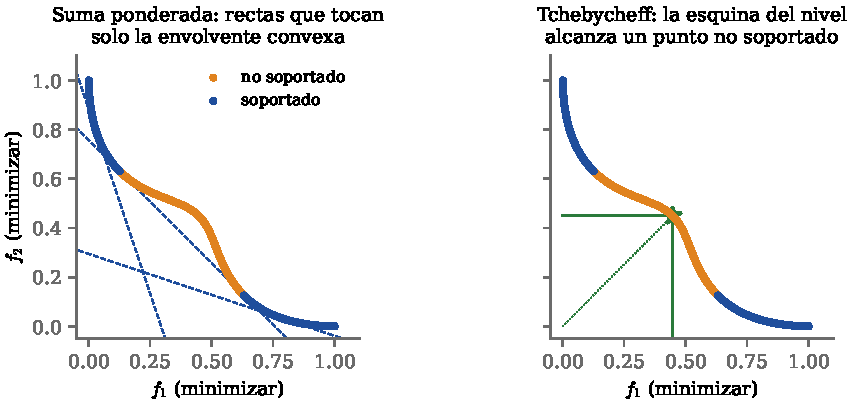
\includegraphics[width=0.95\linewidth]{figs/legendre.pdf}
\caption{Un frente de dos objetivos con una ``abolladura''. Izquierda: cada suma ponderada es una
recta que se desliza hasta tocar el frente; solo toca la envolvente convexa (azul), nunca la parte
naranja. Derecha: la escalarización de Tchebycheff, $\max_i w_i(f_i - z_i)$, tiene curvas de nivel
en forma de esquina; con los pesos adecuados, la esquina alcanza cualquier punto de Pareto,
incluidos los no soportados.}
\label{fig:legendre}
\end{figure}

\subsection{Dos propiedades útiles}

\begin{enumerate}
\item \textbf{Invariancia de escala.} Si cada objetivo se reescala como $f_i \to \alpha_i f_i +
  \beta_i$ con $\alpha_i > 0$, los puntos soportados no cambian (los pesos se reabsorben,
  ejercicio~\ref{ej:escala}). Por eso normalizar por $\Pmax$ o $\Delta P(\Pmax)$ no altera nada.
\item \textbf{Tchebycheff lo alcanza todo.} Con punto ideal $z$ y pesos
  $w_i \propto 1/(f_i(p) - z_i)$, cualquier punto de Pareto $p$ minimiza $\max_i w_i(f_i - z_i)$
  (ejercicio~\ref{ej:tcheby}). Por eso MOEA/D con Tchebycheff no sufre el problema.
\end{enumerate}

\subsection{El test numérico de soporte}

Con un frente muestreado (miles de puntos), ¿cómo saber si un punto es soportado? Se resuelve el
programa lineal
\begin{equation}
s^*(p) = \min_{w\ge0,\ \sum w_i = 1}\ \max_{q\in\mathcal{F}}\ w\cdot\bigl(f(p) - f(q)\bigr).
\label{eq:gap}
\end{equation}
Si $s^* = 0$, existe un peso para el que $p$ es el mejor: soportado. Si $s^* > 0$, para todo peso
hay algún $q$ mejor que $p$, y $s^*$ mide cuánto le falta (en unidades normalizadas). Se escribe como
LP introduciendo la variable $s$: minimizar $s$ sujeto a $w\cdot(f(p)-f(q)) \le s$ para todo $q$.
Usamos tolerancia $s^* > 10^{-3}$ para declarar ``no soportado''. Es \code{support\_gap} en
\code{otto/analysis.py}.

%======================================================================
\section{El resultado central: silla contra tazón}
\label{sec:prop}
%======================================================================

\subsection{Enunciado}

\begin{proposicion}
\label{prop}
Supongamos que
\begin{itemize}
\item[\textbf{(H1)}] el frente de Pareto satura la TUR, $\Delta P = g(P,\eta)$ con $g$ dada por la
  ec.~\eqref{eq:g}, y
\item[\textbf{(H2)}] el frente es una región \emph{bidimensional} de esa superficie: potencia y
  eficiencia se pueden variar de forma independiente (el dominio $D$ de $(P,\eta)$ tiene interior).
\end{itemize}
Entonces:
\begin{enumerate}
\item[(i)] en las variables $f = (-P,-\eta,\Delta P)$, \textbf{ningún punto interior del frente es
  soportado};
\item[(ii)] en las variables $f = (-P,\Delta P,\Sigma)$ la misma superficie es la gráfica de
  $h(P,\Sigma) = 2P^2/\Sigma$, que es \textbf{convexa}. Si el dominio en el plano $(P,\Sigma)$ es
  convexo, todo punto es soportado, aunque de forma \textbf{degenerada}: cada suma ponderada que lo
  soporta tiene un segmento entero de óptimos a lo largo de un rayo $P\propto\Sigma$.
\end{enumerate}
\end{proposicion}

\subsection{Demostración de (i): la silla}

Supongamos que un punto interior $(P_0,\eta_0)$ minimiza
$\phi(P,\eta) = -w_1P - w_2\eta + w_3\,g(P,\eta)$.
\begin{itemize}
\item Si $w_3 = 0$, $\phi$ es lineal y no constante; una función lineal no tiene mínimos en el
  interior de un conjunto abierto. Contradicción. Luego $w_3 > 0$.
\item Con $w_3 > 0$, un mínimo interior exige (condición necesaria de segundo orden) que el
  hessiano de $\phi$, que es $w_3\nabla^2 g$, sea semidefinido positivo.
\end{itemize}
Calculemos el hessiano de $g = 2T_c\,\eta P/(\etaC - \eta)$:
\begin{equation}
g_{PP} = 0,\qquad
g_{P\eta} = \frac{2T_c\,\etaC}{(\etaC-\eta)^2},\qquad
g_{\eta\eta} = \frac{4T_c\,\etaC\,P}{(\etaC-\eta)^3},
\end{equation}
\begin{equation}
\det\nabla^2 g = g_{PP}\,g_{\eta\eta} - g_{P\eta}^2 = -\frac{4T_c^2\,\etaC^2}{(\etaC-\eta)^4} < 0 .
\end{equation}
Un determinante negativo significa un autovalor positivo y uno negativo: el hessiano es
\emph{indefinido}. Contradicción. \hfill$\square$

\paragraph{Intuición.} A $\eta$ fija, $\Delta P$ es \emph{proporcional} a $P$: una recta, curvatura
cero. Pero la pendiente de esa recta, $2T_c\eta/(\etaC-\eta)$, crece con $\eta$. Una superficie que
es recta en una dirección y ``se tuerce'' al moverse en la otra es, localmente, como $z = xy$: el
paraboloide hiperbólico, la silla de montar clásica (Fig.~\ref{fig:silla}, izquierda). Un plano no
puede apoyarse en una silla sin cortarla.

\begin{figure}[h]
\centering
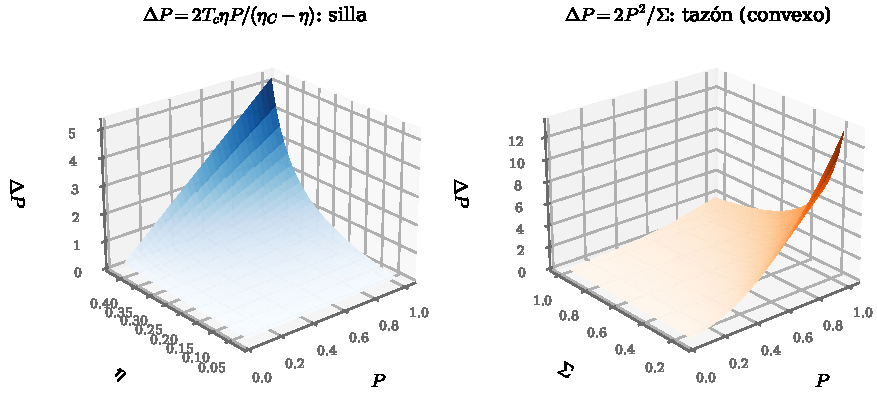
\includegraphics[width=0.95\linewidth]{figs/silla.pdf}
\caption{La misma superficie de saturación de la TUR en dos sistemas de coordenadas. Izquierda:
$(P,\eta,\Delta P)$, una silla (rectas en la dirección de $P$ con pendiente que crece con $\eta$).
Derecha: $(P,\Sigma,\Delta P)$, un tazón convexo, plano a lo largo de los rayos $P\propto\Sigma$.}
\label{fig:silla}
\end{figure}

\subsection{Demostración de (ii): el tazón}

Sustituyendo $\eta = \etaC P/(P+T_c\Sigma)$ (ec.~\ref{eq:sigma}) en $g$:
\[
\frac{2T_c\,\eta}{\etaC-\eta} = \frac{2T_c\cdot\etaC P/(P+T_c\Sigma)}{\etaC T_c\Sigma/(P+T_c\Sigma)}
= \frac{2P}{\Sigma}
\quad\Longrightarrow\quad
\Delta P = \frac{2P^2}{\Sigma}.
\]
(Es simplemente la TUR \eqref{eq:tur} con igualdad.) La función $h(P,\Sigma) = 2P^2/\Sigma$ es la
\emph{perspectiva} de $2P^2$, una construcción que preserva la convexidad (Boyd y Vandenberghe). Su
hessiano,
\begin{equation}
\nabla^2 h = \frac{4}{\Sigma^3}\begin{pmatrix}\Sigma^2 & -P\Sigma\\ -P\Sigma & P^2\end{pmatrix},
\qquad \operatorname{tr} > 0,\quad \det = 0,
\end{equation}
es semidefinido positivo, con dirección nula $(P,\Sigma)$. Para una función convexa, el plano
tangente en cualquier punto queda por debajo de toda la gráfica, así que soporta el punto. Los pesos
correspondientes para $(-P,\Delta P,\Sigma)$ son proporcionales a
$\bigl(\partial_P h,\ 1,\ -\partial_\Sigma h\bigr) = \bigl(4P/\Sigma,\ 1,\ 2P^2/\Sigma^2\bigr)$, todos no
negativos, como debe ser. \hfill$\square$

\subsection{Por qué importan las dos hipótesis}

\begin{itemize}
\item \textbf{Sin (H1)}, la superficie no es la de la ec.~\eqref{eq:g} y no hay razón para la silla.
  Lo veremos en el modelo de control por tramos (sección~\ref{sec:tramos}).
\item \textbf{Sin (H2)}, el frente es una \emph{curva} sobre la silla. Una curva puede estar contenida
  en una silla y aun así ser completamente soportada (piense en una recta trazada sobre $z=xy$). Es
  lo que pasa en respuesta lineal (sección~\ref{sec:lr}).
\end{itemize}
Además, la proposición no dice nada del \emph{borde} del frente: ahí puede haber puntos soportados,
y en la práctica los soportados en $(P,\eta,\Delta P)$ están en partes del borde.

\paragraph{Verificación simbólica.} \code{scripts/geometria.py} calcula estos hessianos con
\texttt{sympy} y aplica el test de soporte a una superficie sintética que satura la TUR: en
$(P,\eta,\Delta P)$ el 85--86\% de los puntos no es soportado (solo bordes); en $(P,\Delta P,\Sigma)$,
0\%.

%======================================================================
\section{La conexión con mecánica estadística}
\label{sec:legendre}
%======================================================================

Esta sección no es necesaria para el resultado, pero es la mejor forma de entenderlo con lo que
sabes del curso.

\subsection{La suma ponderada es una transformada de Legendre}

Maximizar una figura de mérito lineal sobre el frente,
\begin{equation}
F^*(a) = \max_{p\in\mathcal{F}}\ \bigl(a_1 P + a_2\eta - a_3\Delta P\bigr),
\end{equation}
es calcular la \textbf{transformada de Legendre--Fenchel} del frente (su ``función soporte''). Los
pesos son las variables conjugadas. Y la transformada de Legendre tiene una propiedad conocida:
\emph{solo ve la envolvente convexa}. Si transformas dos veces, no recuperas la función original
sino su envolvente convexa.

\subsection{Inequivalencia de ensambles y construcción de Maxwell}

En mecánica estadística pasa exactamente lo mismo al ir del ensamble microcanónico al canónico. La
energía libre es una transformada de Legendre de la entropía:
\begin{equation}
\beta F(\beta) = \min_E\ \bigl(\beta E - S(E)\bigr).
\end{equation}
Si $S(E)$ es cóncava, cada temperatura selecciona una energía y los dos ensambles son
equivalentes. Si $S(E)$ tiene una parte no cóncava (una transición de primer orden, o sistemas con
interacciones de largo alcance), \emph{ninguna temperatura selecciona esas energías}: el ensamble
canónico se las salta y ``rellena'' con la envolvente cóncava. Es la \textbf{construcción de
Maxwell}, y en sistemas de largo alcance se llama \textbf{inequivalencia de ensambles}.

\begin{center}
\begin{tabular}{ll}
\toprule
\textbf{Mecánica estadística} & \textbf{Optimización del motor}\\
\midrule
entropía microcanónica $S(E)$ & frente de Pareto\\
temperatura $\beta$ (variable conjugada) & pesos $(a,b,c)$ de la figura de mérito\\
energía libre $F(\beta)$ (Legendre) & figura de mérito óptima $F^*(a,b,c)$\\
estados que el canónico no selecciona & puntos no soportados\\
construcción de Maxwell & envolvente convexa del frente\\
\bottomrule
\end{tabular}
\end{center}

\begin{idea}[La misma idea, en una frase]
Una figura de mérito lineal es un ``ensamble canónico'' sobre los motores: los pesos hacen de
temperatura. Igual que el ensamble canónico no ve los estados de una región no cóncava de
$S(E)$, la suma ponderada no ve los motores de una región no convexa del frente.
\end{idea}

\subsection{La degeneración en $\Sigma$ es extensividad}

La función $h(P,\Sigma) = 2P^2/\Sigma$ es \textbf{homogénea de grado 1}: $h(\lambda P,\lambda\Sigma) =
\lambda\,h(P,\Sigma)$. Físicamente: dos motores idénticos funcionando en paralelo tienen el doble de
potencia, el doble de producción de entropía y el doble de varianza (si son independientes). Es
\textbf{extensividad}. Una función homogénea de grado 1 es lineal a lo largo de los rayos desde el
origen, y por eso su hessiano tiene un autovalor cero en esa dirección.

Es exactamente lo que pasa con $S(U,V,N)$, también homogénea de grado 1 (relación de Euler): su
hessiano es singular en la dirección $(U,V,N)$. En termodinámica eso no causa problemas; en la suma
ponderada causa \emph{degeneración}: el óptimo no es único a lo largo de cada rayo, y un algoritmo
basado en suma ponderada tiende a amontonar soluciones. Lo veremos en los números (MOEA/D-WS
devuelve solo 68 soluciones distintas de 105).

\subsection{La convexidad depende de las variables}

En el curso se ve que $S(U,V,N)$ es cóncava en sus variables \emph{extensivas naturales}. Escrita
en otras variables (por ejemplo, intensivas) puede dejar de serlo; por eso los potenciales
termodinámicos se definen con transformadas de Legendre y no con cambios de variable arbitrarios.
Nuestro resultado es la versión ``frente de Pareto'' de esa lección: $(P,\Delta P,\Sigma)$ son
cantidades extensivas en el tiempo (tasas que se suman), mientras que $\eta = W/Q_h$ es un
\emph{cociente}, una variable intensiva. Usar un cociente como coordenada rompe la convexidad.

\subsection{Una generalización (derivada para esta guía, por verificar con cuidado)}

La silla no depende de la forma exacta de la TUR. Si el frente es cualquier superficie de la forma
$\Delta P = P\,\varphi(\eta)$ con $\varphi'\neq0$ (fluctuaciones proporcionales a la potencia a
eficiencia fija), entonces
\begin{equation}
\nabla^2(P\varphi) = \begin{pmatrix}0 & \varphi'\\ \varphi' & P\varphi''\end{pmatrix},\qquad
\det = -\varphi'^2 < 0 .
\end{equation}
Siempre es una silla. En variables $(P,\Sigma)$, como $\eta$ depende solo de $t = P/\Sigma$, se tiene
$\Delta P = \Sigma\,\chi(t)$ con $\chi(t) = t\,\varphi(\eta(t))$: la perspectiva de $\chi$, que es
convexa si y solo si $\chi$ lo es. Para la TUR, $\varphi(\eta(t)) = 2t$ y $\chi(t) = 2t^2$. Esto
podría convertir la proposición en un criterio general; es una línea abierta para el paper.

%======================================================================
\section{El límite de respuesta lineal}
\label{sec:lr}
%======================================================================

\subsection{Onsager}

Cerca del equilibrio, los flujos son lineales en las fuerzas termodinámicas:
\begin{equation}
J_1 = L_{11}A_1 + L_{12}A_2,\qquad J_2 = L_{12}A_1 + L_{22}A_2 ,
\end{equation}
con $L$ simétrica (reciprocidad de Onsager) y semidefinida positiva (segunda ley). Para un motor, el
par 2 es el flujo de calor impulsado por la diferencia de temperaturas y el par 1 es el trabajo
contra una fuerza externa. La producción de entropía es $\Sigma = A_1J_1 + A_2J_2$, la potencia
$P = -A_1J_1$ (con $T=1$), la eficiencia relativa a Carnot $\bar\eta = \eta/\etaC = -A_1J_1/(A_2J_2)$,
y la varianza de la potencia (Green--Kubo) $\sigma_P^2 = 2A_1^2L_{11}$.

El acoplamiento se mide con $q = L_{12}/\sqrt{L_{11}L_{22}}\in[-1,1]$; $|q| = 1$ es
\textbf{acoplamiento fuerte} (máquina endorreversible).

\subsection{Todo depende de un solo número}

Almanza-Marrero, Roldán y Manzano (2026) obtienen frentes exactos en este régimen maximizando una suma
ponderada que \emph{incluye} $\eta$. ¿Contradice eso nuestra proposición? No. Fijando los recursos
$A_2 = L_{22} = T = 1$ y definiendo $y = \sqrt{L_{11}}\,A_1$:
\begin{equation}
P = -y(y+q),\qquad \bar\eta = \frac{-y(y+q)}{1+qy},\qquad \Sigma = 1 + 2qy + y^2,\qquad \sigma_P^2 = 2y^2 .
\end{equation}
Las cuatro cantidades dependen solo de $(y,q)$. A $y$ fijo, aumentar $q$ aumenta $P$ y $\bar\eta$ y
disminuye $\Sigma$ (ejercicio~\ref{ej:lr}), así que el frente está en $q = 1$. Con $e = -y\in[0,1]$:
\begin{equation}
P = e(1-e),\qquad \bar\eta = e,\qquad \Sigma = (1-e)^2,\qquad \sigma_P^2 = 2e^2 .
\end{equation}
El frente es una \textbf{curva} de un parámetro, $P = 4\Pmax\,\bar\eta(1-\bar\eta)$, y satura la TUR
exactamente: $\sigma_P^2\Sigma = 2e^2(1-e)^2 = 2P^2$. Cumple (H1) pero no (H2).

Maximizar la figura de mérito sobre $e$ es un problema cuadrático cóncavo cuyo óptimo recorre todo
$[0,1]$ al variar los pesos: la suma ponderada es \textbf{exacta}. \code{scripts/almanza.py} lo
verifica con $2\times10^5$ diseños aleatorios: el 99.95\% del frente tiene $q = 1$, el error contra
la curva analítica es $<2\times10^{-5}$, y no hay ningún punto no soportado.

\begin{figure}[h]
\centering
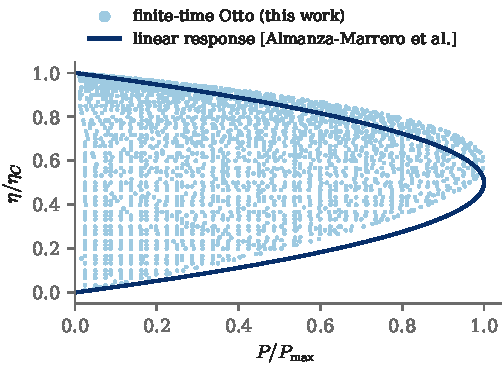
\includegraphics[width=0.55\linewidth]{figs/fig4_linear_response.pdf}
\caption{Frente del Otto en tiempo finito proyectado en $(P,\eta)$ (puntos, bidimensional) y frente
de respuesta lineal (curva). Cada uno normalizado por su propia potencia máxima: la figura compara
dimensiones, no cotas.}
\label{fig:lr}
\end{figure}

\begin{idea}
Cerca del equilibrio hay un solo grado de libertad efectivo: potencia y eficiencia van amarradas.
Lejos del equilibrio se desacoplan, el frente gana una dimensión, y si además satura la TUR, la
suma ponderada con $\eta$ pierde casi todo el interior. El problema aparece justo en el régimen
que motiva optimizar numéricamente.
\end{idea}

%======================================================================
\section{Resultados en el motor de Otto}
\label{sec:otto}
%======================================================================

\subsection{El frente cumple las dos hipótesis}

El frente de referencia del Otto se construyó uniendo un barrido denso de las cuatro variables con
todas las corridas de los algoritmos, y quedándose con los no dominados (unos 4\,800 puntos tras
adelgazar en una grilla de vóxeles). Sobre él:
\begin{itemize}
\item \textbf{(H1)}: mediana $\xi = 0.996$, máximo $1.005$. Satura la TUR.
\item \textbf{(H2)}: $\omega_h$, $r$ y los tiempos permiten mover $P$ y $\eta$ por separado; el
  frente llena una región del plano $(P,\eta)$ (Fig.~\ref{fig:lr}).
\end{itemize}
Y la predicción se cumple: el \textbf{91\%} del frente no es soportado en $(P,\eta,\Delta P)$, con
brechas de hasta $0.077$; en $(P,\Delta P,\Sigma)$ solo el \textbf{4\%}, con brechas menores que
$0.005$.

\subsection{El costo físico: ¿cuánto pierde un diseñador?}

La brecha $s^*$ es geométrica. Para traducirla a física (\code{scripts/costo\_fisico.py}), sea $S$ el
conjunto de motores alcanzables con una figura de mérito lineal (los soportados) y $p$ un motor del
frente. Definimos la \textbf{pérdida}
\begin{equation}
\varepsilon(p) = \min_{s\in S}\ \max\!\left(\frac{P_p}{P_s},\ \frac{\eta_p}{\eta_s},\
\frac{\Delta P_s}{\Delta P_p}\right) - 1 .
\end{equation}
Se lee así: el mejor motor que el diseñador puede obtener es, como mínimo, un $\varepsilon$ peor que
$p$ en algún objetivo (menos potencia, menos eficiencia o más fluctuaciones, en términos relativos).

\begin{center}
\begin{tabular}{lcc}
\toprule
Figura de mérito lineal en & $(P,\eta,\Delta P)$ & $(P,\Delta P,\Sigma)$\\
\midrule
fracción del frente alcanzable & 11\% & 98\% \\
pérdida $\varepsilon$ mediana & 14\% & 0\% \\
frente con $\varepsilon > 5\%$ & 75\% & 7\% \\
frente con $\varepsilon > 10\%$ & 60\% & 3\% \\
\bottomrule
\end{tabular}
\end{center}

\begin{figure}[h]
\centering
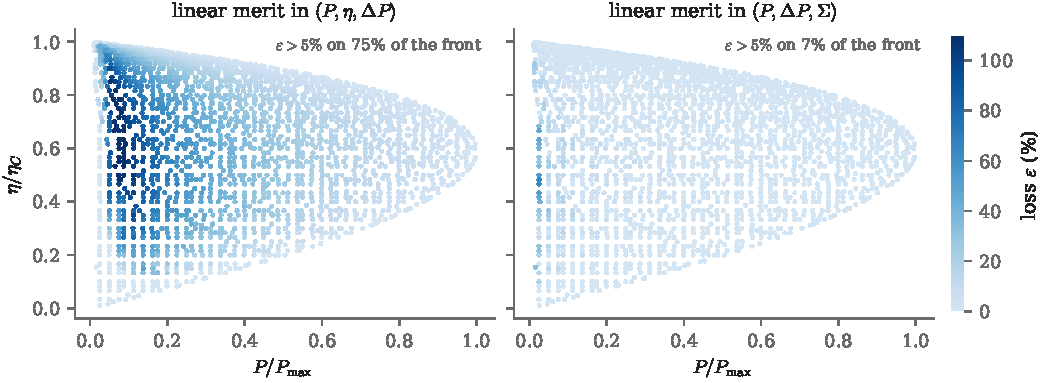
\includegraphics[width=\linewidth]{figs/fig2_cost.pdf}
\caption{Cada punto es un motor del frente en el plano $(P/\Pmax,\eta/\etaC)$, coloreado por la
pérdida $\varepsilon$. Izquierda: figura de mérito lineal en $\eta$. Derecha: en $\Sigma$.}
\label{fig:costo}
\end{figure}

\paragraph{Dónde se pierde.} Las pérdidas grandes se concentran a \textbf{baja potencia y eficiencia
media o alta} (mediana $P/\Pmax = 0.34$, $\eta/\etaC = 0.68$ entre los puntos con $\varepsilon > 5\%$):
los motores lentos, eficientes y de poco ruido. \textbf{Ejemplo extremo:} el motor con
$P/\Pmax = 0.075$ y $\eta/\etaC = 0.55$. Lo mejor que se puede obtener con una figura de mérito lineal
en $\eta$ tiene $\eta/\etaC = 0.24$ y $2.3$ veces sus fluctuaciones.

\paragraph{La recomendación física.} Escribir la figura de mérito con $\Sigma$ (como hacen Erdman
\emph{et al.}) recupera casi todo el frente de eficiencia.

\subsection{Los algoritmos y la descomposición de la pérdida}

Se compararon siete algoritmos evolutivos (sección~\ref{sec:algos}) con 30 semillas y $42\,000$
evaluaciones cada uno. La métrica principal es el \textbf{hipervolumen} (HV): el volumen del espacio
de objetivos dominado por las soluciones encontradas, hasta un punto de referencia. Más es mejor.

Para separar las dos razones por las que una suma ponderada puede perder HV, calculamos el HV de los
puntos soportados del frente de referencia. Es el \textbf{techo} de cualquier método de suma
ponderada, con los pesos que sea. Entonces:
\begin{itemize}
\item \textbf{pérdida por alcanzabilidad} $=$ HV(referencia) $-$ techo: lo que ningún peso recupera;
\item \textbf{pérdida por reparto} $=$ techo $-$ HV(MOEA/D-WS): lo que se pierde por cómo los pesos
  reparten las soluciones.
\end{itemize}

\begin{center}
\begin{tabular}{lcc}
\toprule
Otto, 30 semillas & $(P,\eta,\Delta P)$ & $(P,\Delta P,\Sigma)$\\
\midrule
HV del frente de referencia & 1.0810 & 1.2114\\
techo de cualquier suma ponderada & \textbf{0.9950} & 1.2113\\
\midrule
SMS-EMOA & 1.0425 & 1.1868\\
MOEA/D-AWA & 1.0404 & 1.1829\\
MOEA/D (Tchebycheff) & 1.0385 & 1.1744\\
NSGA-III & 1.0310 & 1.1700\\
RVEA & 1.0269 & 1.1683\\
NSGA-II & 1.0073 & 1.1612\\
MOEA/D-WS (suma ponderada) & 0.9670 & 1.1220\\
\midrule
pérdida WS: alcanzabilidad $+$ reparto & $\mathbf{0.086} + 0.028$ & $0.0001 + \mathbf{0.089}$\\
\bottomrule
\end{tabular}
\end{center}

\begin{idea}[Cómo leer la tabla]
La suma ponderada queda última en ambas formulaciones y pierde un HV parecido, pero \emph{por razones
distintas}. Con $\eta$, casi toda la pérdida es de alcanzabilidad: la silla. Seis de los siete
algoritmos, incluso NSGA-II, superan el techo de cualquier suma ponderada. Con $\Sigma$, la
alcanzabilidad es perfecta y toda la pérdida es de reparto: la degeneración por extensividad
(68 soluciones distintas de 105). La proposición predice exactamente esas dos cosas.
\end{idea}

\begin{figure}[h]
\centering
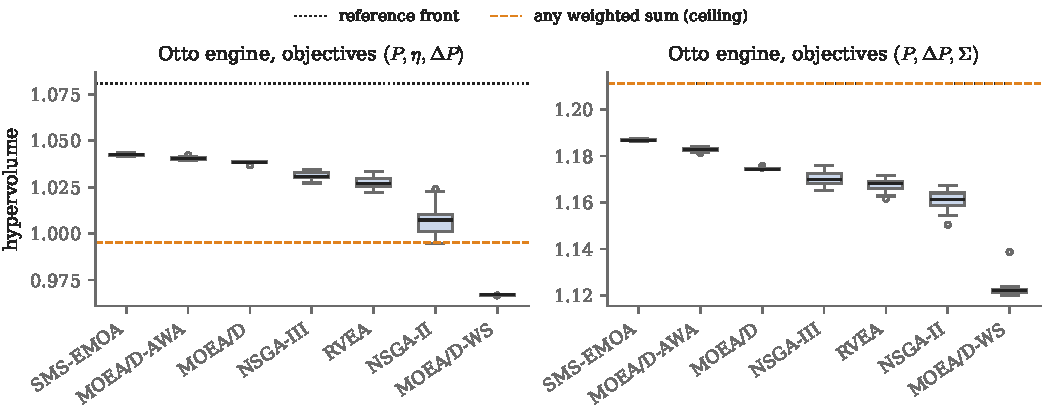
\includegraphics[width=\linewidth]{figs/fig3_hv_otto.pdf}
\caption{HV de los siete algoritmos en el Otto. Punteada: frente de referencia. Discontinua: techo
de cualquier suma ponderada. Con $\eta$ (izquierda) el techo queda por debajo de seis algoritmos;
con $\Sigma$ (derecha) coincide con la referencia.}
\end{figure}

%======================================================================
\section{Cuando la TUR se rompe: control por tramos}
\label{sec:tramos}
%======================================================================

\subsection{El modelo de Erdman}

Para ver qué pasa sin (H1) usamos el motor de punto cuántico de Erdman \emph{et al.} (2023):
$H(t) = u(t)E_0\sigma_z/2$, con relajación $\dot p = -\gamma\bigl[p - f(\beta(t)E_0u(t))\bigr]$,
$f(x) = 1/(1+e^x)$ (la misma forma de Gibbs/Fermi de la sección 2). Parámetros: $\beta_H = 1$,
$\beta_C = 2$, $E_0 = 2.5$, $u\in[0.2,1.1]$, $\gamma = 1$. El ciclo de duración $\tau$ se divide en
$N = 8$ tramos iguales; en cada uno se elige $u_k$ y \emph{con qué baño} se conecta. Son 17
variables (8 controles, 8 elecciones de baño y $\tau$). El Otto de cuatro tramos es un caso
particular, y el código lo reproduce con error $10^{-9}$ (\code{otto/piecewise.py}).

\subsection{Qué se observa}

\begin{itemize}
\item \textbf{La TUR se viola fuertemente}: el 81\% del frente tiene $\xi > 1$, con $\xi$ hasta
  $4$. El control libre permite ciclos que la cota estacionaria no cubre.
\item \textbf{La silla desaparece}: aunque el test marca como no soportado el 31\% ($\Sigma$) y el
  48\% ($\eta$) del frente, las brechas son diminutas (mediana $\approx 0.003$), y el techo de la
  suma ponderada queda a $0.1\%$ ($\Sigma$) y $0.2\%$ ($\eta$) del HV de referencia. El frente es
  casi convexo en ambas variables.
\item La suma ponderada sigue rindiendo distinto en $\eta$ que en $\Sigma$ (en $\Sigma$ queda segunda,
  detrás de SMS-EMOA), pero su pérdida ahora es \emph{toda de reparto}; la proposición no la explica.
\end{itemize}

\begin{center}
\begin{tabular}{lcc}
\toprule
Tramos, 30 semillas, 315\,000 evaluaciones & $(P,\eta,\Delta P)$ & $(P,\Delta P,\Sigma)$\\
\midrule
$\xi$ (mediana / máximo) & 1.59 / 4.04 & 1.45 / 4.02\\
HV referencia / techo & 1.1208 / 1.1184 & 1.2284 / 1.2276\\
SMS-EMOA / MOEA/D-AWA / MOEA/D-WS & 1.085 / 1.065 / 1.059 & 1.209 / 1.187 / 1.193\\
pérdida WS: alcanzabilidad $+$ reparto & $0.0024 + 0.060$ & $0.0008 + 0.035$\\
\bottomrule
\end{tabular}
\end{center}

\begin{idea}
El efecto geométrico está ligado a la saturación de la TUR: fuerte en el Otto (la alcanzabilidad se
lleva el 8\% del HV) y despreciable cuando el control libre rompe la cota. No es que ``la
suma ponderada con $\eta$ siempre falle'': falla cuando el frente es una superficie que satura la
TUR. Cómo interpola el efecto entre $\xi = 1$ y $\xi \gg 1$ es una pregunta abierta.
\end{idea}

%======================================================================
\section{Los algoritmos evolutivos}
\label{sec:algos}
%======================================================================

Esta parte es tu especialidad, así que va resumida y centrada en lo que importa para el argumento.

\subsection{Los siete algoritmos}

Todos usan población $N = 105$ (pesos de Das--Dennis con 13 divisiones para tres objetivos), cruce
SBX (probabilidad 1, $\eta_c = 20$) y mutación polinomial ($\eta_m = 20$).
\begin{itemize}
\item \textbf{NSGA-II}: ordenamiento no dominado más distancia de crowding; elitista.
\item \textbf{NSGA-III}: reemplaza el crowding por asociación a direcciones de referencia.
\item \textbf{SMS-EMOA}: estado estacionario; descarta el individuo con menor contribución al
  hipervolumen. Optimiza directamente la métrica con la que se evalúa, por eso suele ganar en HV.
\item \textbf{RVEA}: vectores de referencia con distancia penalizada por ángulo.
\item \textbf{MOEA/D}: descompone el problema en $N$ subproblemas escalares, uno por vector de pesos
  $w$, resueltos en paralelo con vecindarios (10\% de $N$, $\delta = 0.9$, $n_r = 2$). Usa
  \textbf{Tchebycheff normalizado}:
  \[ g^{\mathrm{te}}(x\mid w) = \max_i\ w_i\,\frac{f_i(x) - z_i^*}{z_i^{\mathrm{nad}} - z_i^*}. \]
\item \textbf{MOEA/D-AWA} (Qi \emph{et al.} 2014): MOEA/D más ajuste adaptativo de pesos. Transforma
  los pesos ($w_i \to (1/w_i)/\sum_j 1/w_j$) para que las direcciones de Tchebycheff queden uniformes,
  mantiene una población externa de no dominados (hasta $1.5N$) y, después del 80\% de la corrida,
  cada 10 generaciones elimina el 5\% de subproblemas en las zonas más pobladas y crea otros en las
  zonas más vacías (medidas con el producto de distancias a los vecinos más cercanos).
\item \textbf{MOEA/D-WS}: igual que MOEA/D pero con suma ponderada $g = \sum_i w_i\bar f_i$. Es la
  versión evolutiva de ``barrer los pesos de una figura de mérito lineal'': la línea base que el
  argumento necesita.
\end{itemize}

\subsection{Métricas y estadística}

\begin{itemize}
\item \textbf{HV}: volumen dominado, en coordenadas normalizadas por el frente de referencia, con
  punto de referencia $1.1$ en cada eje.
\item \textbf{IGD+}: distancia media desde los puntos del frente de referencia hasta la solución más
  cercana, contando solo las componentes en las que la solución es peor
  ($d^+(z,a) = \sqrt{\sum_i\max(a_i - z_i, 0)^2}$). Menos es mejor. MOEA/D-AWA tiene el mejor IGD+
  en el Otto en ambas formulaciones.
\item \textbf{Mann--Whitney U}: test no paramétrico (por rangos) para comparar las 30 corridas de cada
  algoritmo con MOEA/D-AWA.
\item \textbf{Holm}: corrección por comparaciones múltiples (seis tests). Se ordenan los $p$ y se
  multiplican por $(m - \text{rango})$, forzando monotonía. En el Otto todas las diferencias dan
  $p = 1.8\times10^{-10}$: separación completa de las 30 corridas (ninguna corrida de un algoritmo
  supera a ninguna del otro), que es el mínimo posible tras la corrección.
\end{itemize}

\subsection{Lo que pasó con DCE-MOEA/D}

Antes de esto se probó tu DCE-MOEA/D (en C++) en el Otto, con y sin el AWA de Qi. Su rendimiento
fue equivalente a MOEA/D-DE con el mismo AWA: la mejora venía del AWA, no del genotipo de gradiente.
Por eso el proyecto quedó con MOEA/D + AWA de Qi en Python.

%======================================================================
\section{Qué es nuevo, qué no, y qué diría un revisor}
%======================================================================

\paragraph{Ya se sabía.}
\begin{itemize}
\item Que la suma ponderada solo encuentra la envolvente convexa (desde los años 90).
\item Que los ciclos de Otto rápidos saturan la TUR (Erdman \emph{et al.} 2023).
\item Que los motores cíclicos pueden violar la TUR estacionaria (Holubec y Ryabov 2018).
\item Los frentes exactos en respuesta lineal (Almanza-Marrero \emph{et al.} 2026).
\end{itemize}

\paragraph{Lo que aporta el proyecto.}
\begin{itemize}
\item La conexión: saturación de la TUR $+$ frente bidimensional $\Rightarrow$ silla en $(P,\eta,\Delta P)$
  y tazón en $(P,\Delta P,\Sigma)$. Con demostración.
\item El costo físico medido en un modelo estándar (11\% alcanzable, 14\% de pérdida mediana).
\item La explicación de por qué la suma ponderada es exacta en respuesta lineal (el frente es una
  curva).
\item La descomposición alcanzabilidad/reparto, que separa la silla (con $\eta$) de la degeneración
  por extensividad (con $\Sigma$).
\end{itemize}

\paragraph{Críticas esperables.}
\begin{enumerate}
\item ``Es un corolario directo de un resultado clásico.'' Defensa: la generalización a
  $\Delta P = P\varphi(\eta)$ (sección~\ref{sec:legendre}) y el costo físico.
\item ``¿Quién comete el error?'' Erdman usa $\Sigma$ (bien); Almanza usa $\eta$ pero en respuesta
  lineal (donde es exacto). Hace falta encontrar trabajos que usen $\eta$ en una suma ponderada
  lejos del equilibrio.
\item ``El efecto depende de (H1), que es frágil'': con control libre desaparece.
\item ``El modelo no es cuántico'': no hay coherencias; el qubit es una cadena de Markov clásica. Lo
  cuántico es solo la discretización de niveles.
\end{enumerate}

%======================================================================
\section{Mapa del código y cómo reproducir}
%======================================================================

\begin{center}
\small
\begin{tabular}{p{0.36\linewidth}p{0.56\linewidth}}
\toprule
\textbf{Archivo} & \textbf{Qué hace (sección de esta guía)}\\
\midrule
\code{otto/model.py} & Gibbs, matrices $M$, ciclo límite, matriz inclinada, $P$, $\Delta P$, $\Sigma$, $\xi$, Monte Carlo (2--5)\\
\code{otto/problem.py} & Problemas de optimización: variables y objetivos $\eta$ o $\Sigma$ (6)\\
\code{otto/piecewise.py} & Modelo de Erdman por tramos (11)\\
\code{otto/moead.py} & MOEA/D, MOEA/D-AWA y MOEA/D-WS (12)\\
\code{otto/analysis.py} & Test de soporte por programación lineal, ec.~\eqref{eq:gap} (6)\\
\code{scripts/geometria.py} & Hessianos con sympy y superficie sintética (7)\\
\code{scripts/costo\_fisico.py} & Pérdida $\varepsilon$ y figura de costo (10)\\
\code{scripts/almanza.py} & Respuesta lineal (9)\\
\code{scripts/run\_piecewise.py} & Corre los 7 algoritmos (\code{--model otto} o tramos) (10--12)\\
\code{scripts/analyze\_piecewise.py} & HV, IGD+, tests, techo de suma ponderada (10--12)\\
\code{scripts/gap\_sensitivity.py} & Sensibilidad a la tolerancia del test (11)\\
\code{paper/make\_figures.py} & Figuras del paper\\
\code{docs/proposicion.md} & La proposición y la evidencia, en español\\
\bottomrule
\end{tabular}
\end{center}

\paragraph{Comandos} (desde \code{\textasciitilde/Projects/hidden-front}, con el entorno del proyecto):
{\small
\begin{verbatim}
.venv/bin/python -m pytest -q                       # 15 tests
.venv/bin/python scripts/geometria.py               # silla vs tazón
.venv/bin/python scripts/run_piecewise.py --model otto --seeds 30 --gens 400 --jobs 24
.venv/bin/python scripts/analyze_piecewise.py --model otto
.venv/bin/python scripts/costo_fisico.py
.venv/bin/python scripts/almanza.py
.venv/bin/python scripts/run_piecewise.py --seeds 30 --gens 3000 --jobs 24
.venv/bin/python scripts/refine_reference.py
.venv/bin/python scripts/analyze_piecewise.py
\end{verbatim}
}

%======================================================================
\section{Ejercicios}
%======================================================================

\newcounter{ejer}
\newcommand{\ejercicio}[2]{\par\medskip\refstepcounter{ejer}\label{#1}\noindent\textbf{Ejercicio \theejer\ (#2).}\ }

\ejercicio{ej:gibbs}{Gibbs} Deduce $a = 1/(1+e^{\omega/T})$ a partir de la función de partición de un
sistema de dos niveles.

\ejercicio{ej:ciclolimite}{ciclo límite} A partir de $p_1 = a_h + (p_2 - a_h)x_h$ y
$p_2 = a_c + (p_1 - a_c)x_c$, deduce $p_1$ y la ec.~\eqref{eq:dp} para $p_1 - p_2$.

\ejercicio{ej:numerico}{números} Con $\omega_h = 2.035$, $\omega_c = 1.433$, $\tau_h = \tau_c = 0.675$,
$\tau_q = 0.05$, $T_h = 1$, $T_c = 0.5$, $\gamma = 1$, calcula $p_1 - p_2$, $W$, $P$, $\eta$ y $\Sigma$.
Con $\Delta P = 0.0126$, calcula $\xi$.

\ejercicio{ej:sigma}{producción de entropía} Demuestra que $\Sigma = P(\etaC - \eta)/(\eta T_c)$.

\ejercicio{ej:tur}{TUR de motores} Partiendo de $\Delta P\,\Sigma \ge 2P^2$, deduce
$\eta \le \etaC/(1 + 2T_cP/\Delta P)$.

\ejercicio{ej:correl}{correlaciones} ¿Por qué $\theta''(0)$ no es igual a la varianza del trabajo de
un solo ciclo? ¿Con qué rapidez decaen las correlaciones entre ciclos?

\ejercicio{ej:hess}{hessianos} Calcula el hessiano de $h(P,\Sigma) = 2P^2/\Sigma$ y muestra que es
semidefinido positivo con dirección nula $(P,\Sigma)$. Verifica que $h$ es homogénea de grado 1.

\ejercicio{ej:escala}{invariancia de escala} Muestra que si $f_i\to\alpha_if_i + \beta_i$ con
$\alpha_i > 0$, los puntos soportados no cambian.

\ejercicio{ej:tcheby}{Tchebycheff} Sea $p$ un punto de Pareto y $z$ un punto ideal con $z_i < f_i(p)$.
Muestra que con $w_i \propto 1/(f_i(p) - z_i)$, $p$ minimiza $\max_i w_i(f_i - z_i)$.

\ejercicio{ej:lr}{respuesta lineal} Con $P = -y(y+q)$, $\bar\eta = -y(y+q)/(1+qy)$ y
$\Sigma = 1+2qy+y^2$, $y\in(-q,0)$, muestra que aumentar $q$ mejora los tres objetivos. Muestra que
con $q = 1$ el frente satura la TUR.

\ejercicio{ej:silla}{intuición} Toma $z = xy$. Muestra que ningún plano $z = \alpha x + \beta y + c$
puede quedar por debajo de la superficie en un entorno de un punto, y que sin embargo la curva
$\{(t,t,t^2)\}$ contenida en ella es convexa. Relaciónalo con (H2).

%======================================================================
\section{Soluciones}
%======================================================================

\textbf{\ref{ej:gibbs}.} $Z = 1 + e^{-\omega/T}$, así que
$p_{\mathrm{eq}} = e^{-\omega/T}/Z = 1/(e^{\omega/T} + 1)$.

\textbf{\ref{ej:ciclolimite}.} Sustituyendo la segunda en la primera:
$p_1 = a_h(1-x_h) + x_h a_c(1-x_c) + x_hx_c\,p_1$, luego
$p_1 = [a_h(1-x_h) + x_ha_c(1-x_c)]/(1 - x_hx_c)$. Además $p_1 - p_2 = (1-x_c)(p_1 - a_c)$ y
$p_1 - a_c = (a_h - a_c)(1-x_h)/(1-x_hx_c)$ (los términos con $a_c$ se agrupan como
$a_c[x_h - x_hx_c - 1 + x_hx_c] = -a_c(1-x_h)$).

\textbf{\ref{ej:numerico}.} $a_h = 0.1156$, $a_c = 0.0539$, $x_h \approx x_c \approx 0.509$.
$p_1 - p_2 = 0.0617\times0.2408/0.7406 = 0.0201$. $W = 0.602\times0.0201 = 0.0121$,
$\tau_{\mathrm{ciclo}} = 1.45$, $P = 0.00833$, $\eta = 1 - 1.433/2.035 = 0.296$,
$\Sigma = 0.0201\,(2.866 - 2.035)/1.45 = 0.0115$.
$\xi = 2P^2/(\Delta P\,\Sigma) = 1.39\times10^{-4}/1.45\times10^{-4} = 0.96$.

\textbf{\ref{ej:sigma}.} En tasas, $\dot Q_h = P/\eta$ y $\dot Q_c = \dot Q_h - P = P(1-\eta)/\eta$.
Entonces $\Sigma = \dot Q_c/T_c - \dot Q_h/T_h = \frac{P}{\eta}\bigl[\frac{1-\eta}{T_c} - \frac{1}{T_h}\bigr]
= \frac{P}{\eta T_c}\bigl[1 - \eta - \frac{T_c}{T_h}\bigr] = \frac{P(\etaC-\eta)}{\eta T_c}$.

\textbf{\ref{ej:tur}.} $\Delta P\,P(\etaC-\eta)/(\eta T_c) \ge 2P^2 \Rightarrow \Delta P(\etaC-\eta)\ge
2T_cP\eta \Rightarrow \eta(\Delta P + 2T_cP) \le \Delta P\,\etaC$, y se divide por $\Delta P$.

\textbf{\ref{ej:correl}.} $v = \operatorname{Var}(w) + 2\sum_{j\ge1}\operatorname{Cov}(w_0,w_j)$: el
estado al final de un ciclo condiciona el siguiente. Las covarianzas decaen con el segundo autovalor
de la matriz de un ciclo, que es $D = x_hx_c$: $\operatorname{Cov}(w_0,w_j)\propto (x_hx_c)^{j}$.
Contactos largos ($x\to0$) borran la memoria; contactos cortos la alargan.

\textbf{\ref{ej:hess}.} $h_{PP} = 4/\Sigma$, $h_{P\Sigma} = -4P/\Sigma^2$, $h_{\Sigma\Sigma} = 4P^2/\Sigma^3$.
Traza positiva y determinante $16P^2/\Sigma^4 - 16P^2/\Sigma^4 = 0$: semidefinido positivo.
$\nabla^2h\,(P,\Sigma)^\top = (4P/\Sigma - 4P/\Sigma,\ -4P^2/\Sigma^2 + 4P^2/\Sigma^2) = 0$.
$h(\lambda P,\lambda\Sigma) = 2\lambda^2P^2/(\lambda\Sigma) = \lambda h$.

\textbf{\ref{ej:escala}.} $\sum_iw_i(\alpha_if_i + \beta_i) = \sum_i(w_i\alpha_i)f_i + \text{cte}$.
Con $w'_i = w_i\alpha_i/\sum_jw_j\alpha_j \ge 0$, el minimizador es el mismo.

\textbf{\ref{ej:tcheby}.} Con esos pesos, $w_i(f_i(p) - z_i) = c$ igual para todo $i$, así que el
valor en $p$ es $c$. Si existiera $q$ con $\max_iw_i(f_i(q) - z_i) < c$, tendríamos
$f_i(q) < f_i(p)$ para todo $i$: $q$ dominaría a $p$, contradicción.

\textbf{\ref{ej:lr}.} $\partial_qP = -y > 0$; $\partial_q\Sigma = 2y < 0$;
$\partial_q\bar\eta = -y(1-y^2)/(1+qy)^2 > 0$ para $y\in(-1,0)$. Con $q = 1$, $e = -y$:
$\sigma_P^2\Sigma = 2e^2(1-e)^2 = 2P^2$.

\textbf{\ref{ej:silla}.} El hessiano de $xy$ es $\bigl(\begin{smallmatrix}0&1\\1&0\end{smallmatrix}\bigr)$,
con autovalores $\pm1$; a lo largo de $x = -y$ la superficie cae por debajo de cualquier plano
tangente. Pero sobre la curva $x = y = t$ vale $z = t^2$, convexa. Una curva sobre una silla puede ser
convexa; por eso (H2) es necesaria. Es lo que pasa en respuesta lineal.

%======================================================================
\section{Glosario}
%======================================================================

\begin{description}[style=nextline,leftmargin=1.2em]
\item[Brecha $\omega$] Diferencia de energía entre los dos niveles del qubit; hace el papel del volumen.
\item[Ciclo límite] Régimen periódico al que llega el qubit tras pocos ciclos.
\item[Estadística de conteo completa] Cálculo de todos los cumulantes de una cantidad acumulada
  (trabajo) con una matriz inclinada.
\item[Función generadora escalada $\theta(\chi)$] $\lim\frac1n\ln\langle e^{\chi W_n}\rangle$; el
  ``$\ln Z$'' del trabajo.
\item[Producción de entropía $\Sigma$] Entropía generada en los baños por unidad de tiempo; cero si y
  solo si el motor es reversible ($\eta = \etaC$).
\item[TUR] $\Delta P\,\Sigma\ge2P^2$: el ruido relativo está acotado por la disipación.
\item[$\xi$] $2P^2/(\Delta P\,\Sigma)$; $\xi = 1$ es saturar la TUR.
\item[Frente de Pareto] Conjunto de compromisos no dominados entre los objetivos.
\item[Punto soportado] Punto del frente que minimiza alguna suma ponderada con pesos no negativos.
\item[Techo de suma ponderada] HV de los puntos soportados: lo máximo que puede lograr un método de
  suma ponderada.
\item[Silla / tazón] Superficie con hessiano indefinido / semidefinido positivo.
\item[Inequivalencia de ensambles] Cuando el ensamble canónico no reproduce estados del
  microcanónico porque $S(E)$ no es cóncava.
\item[Respuesta lineal] Régimen cercano al equilibrio con flujos lineales en las fuerzas (Onsager).
\end{description}

%======================================================================
\section*{Referencias principales}
\addcontentsline{toc}{section}{Referencias principales}
%======================================================================
\begin{itemize}\small
\item A.~C. Barato y U. Seifert, Phys. Rev. Lett. \textbf{114}, 158101 (2015). (TUR)
\item T.~R. Gingrich, J.~M. Horowitz, N. Perunov y J.~L. England, Phys. Rev. Lett. \textbf{116}, 120601 (2016).
\item P. Pietzonka y U. Seifert, Phys. Rev. Lett. \textbf{120}, 190602 (2018). (TUR de motores)
\item V. Holubec y A. Ryabov, Phys. Rev. Lett. \textbf{121}, 120601 (2018). (motores cíclicos)
\item P.~A. Erdman \emph{et al.}, Phys. Rev. Research \textbf{5}, L022017 (2023). (frentes con RL, modelo por tramos)
\item J.~A. Almanza-Marrero, É. Roldán y G. Manzano, arXiv:2603.19885 (2026). (respuesta lineal)
\item F.~L. Curzon y B. Ahlborn, Am. J. Phys. \textbf{43}, 22 (1975).
\item H. Touchette, Phys. Rep. \textbf{478}, 1 (2009). (grandes desviaciones)
\item I. Das y J.~E. Dennis, Struct. Optim. \textbf{14}, 63 (1997). (límites de la suma ponderada)
\item M. Ehrgott, \emph{Multicriteria Optimization}, Springer (2005).
\item S. Boyd y L. Vandenberghe, \emph{Convex Optimization}, Cambridge (2004). (funciones perspectiva)
\item Q. Zhang y H. Li, IEEE Trans. Evol. Comput. \textbf{11}, 712 (2007). (MOEA/D)
\item Y. Qi \emph{et al.}, Evol. Comput. \textbf{22}, 231 (2014). (MOEA/D-AWA)
\end{itemize}


\end{document}
